The phone app layer contains subsystems of Bluetooth, alert notification or history, notification setting, and vibration setting.

\subsection{Log in}
The text written through the app login ID and the information on the mobile phone will be uploaded to the web server and the corresponding value will be stored in the database system. 

\begin{figure}[h!]
	\centering
 	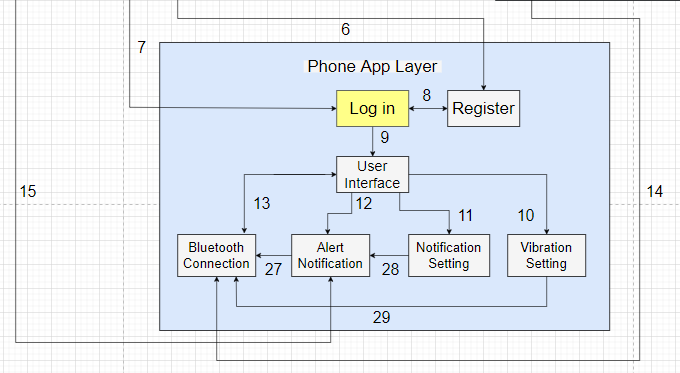
\includegraphics[width=0.60\textwidth]{images/phone_login.png}
 \caption{Phone App Layer diagram}
\end{figure}

\subsubsection{Assumptions}
The user has an android app downloaded on his/her phone and created an account.

\subsubsection{Responsibilities}
This subsystem is responsible for specifying a user and bringing information from the database.

\subsubsection{Subsystem Interfaces}
Each of the inputs and outputs for the subsystem are defined here. Create a table with an entry for each labelled interface that connects to this subsystem. For each entry, describe any incoming and outgoing data elements will pass through this interface.

\begin {table}[H]
\caption {Log in interfaces} 
\begin{center}
    \begin{tabular}{ | p{1cm} | p{6cm} | p{3cm} | p{3cm} |}
    \hline
    ID & Description & Inputs & Outputs \\ \hline
    #7 & From database & \pbox{Database information} & \pbox{User login information}  \\ \hline
    #9 & Login information & \pbox{User ID, User password} & \pbox{User wristband information}  \\ \hline
    #8 & To Registration page & \pbox{Click on the 'Register' button} & \pbox{Registration page}  \\ \hline
    \end{tabular}
\end{center}
\end{table}

\subsection{Register}
The register subsystem will hold new account information and store it in the database. The user’s email address will be the log-in ID and the system will ask the user to verify the email before proceeding.  

\begin{figure}[h!]
	\centering
 	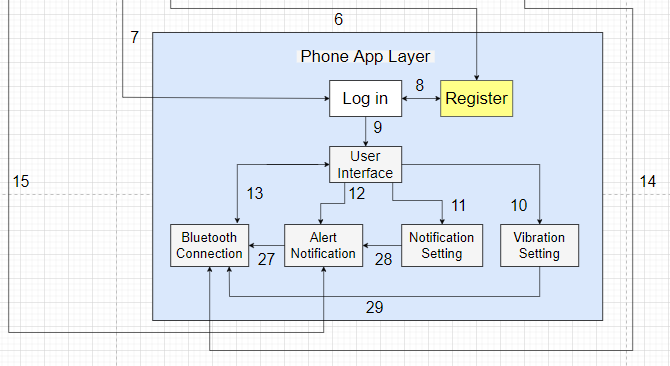
\includegraphics[width=0.60\textwidth]{images/phone_register.png}
 \caption{Phone App Layer diagram}
\end{figure}

\subsubsection{Assumptions}
The user has an android app downloaded on his/her phone and the app has access to the database.

\subsubsection{Responsibilities}
This subsystem is responsible for creating a new account and storing the information in the database so that the user is able to log in.

\subsubsection{Subsystem Interfaces}
Each of the inputs and outputs for the subsystem are defined here. Create a table with an entry for each labelled interface that connects to this subsystem. For each entry, describe any incoming and outgoing data elements will pass through this interface.

\begin {table}[H]
\caption {Register interfaces} 
\begin{center}
    \begin{tabular}{ | p{1cm} | p{6cm} | p{3cm} | p{3cm} |}
    \hline
    ID & Description & Inputs & Outputs \\ \hline
    #6 & User information & \pbox{Name, Email address, Password} & \pbox{App main page}  \\ \hline
    #8 & To previous page & \pbox{Click on the 'Back' button} & \pbox{Log in page}  \\ \hline
    \end{tabular}
\end{center}
\end{table}

\subsection{User interface}
The user interface subsystem will allow user to go to desire settings and make changes.   

\begin{figure}[h!]
	\centering
 	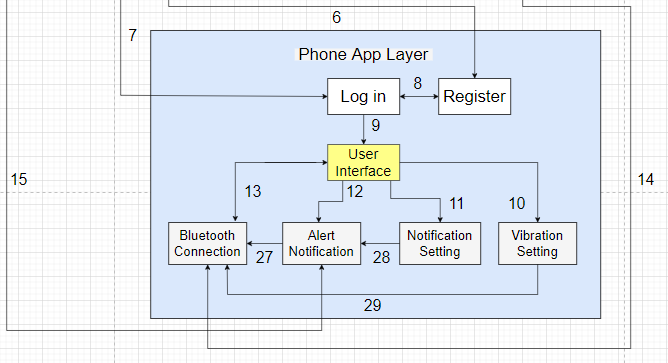
\includegraphics[width=0.60\textwidth]{images/phone_ui.png}
 \caption{Phone App Layer diagram}
\end{figure}

\subsubsection{Assumptions}
It is assumed that the user is already signed in.

\subsubsection{Responsibilities}
This subsystem is responsible for letting user to go to different settings and providing convenience to the user. 

\subsubsection{Subsystem Interfaces}
Each of the inputs and outputs for the subsystem are defined here. Create a table with an entry for each labelled interface that connects to this subsystem. For each entry, describe any incoming and outgoing data elements will pass through this interface.

\begin {table}[H]
\caption {User interfaces} 
\begin{center}
    \begin{tabular}{ | p{1cm} | p{6cm} | p{3cm} | p{3cm} |}
    \hline
    ID & Description & Inputs & Outputs \\ \hline
    #9 & From login & \pbox{User ID, password} & \pbox{Main page}  \\ \hline
    #13 & Bluetooth Connection & \pbox{Click on the 'Bluetooth' button} & \pbox{Bluetooth setting page}  \\ \hline
    #12 & Alert notification & \pbox{Click on the 'History' button} & \pbox{History list}  \\ \hline
    #11 & Notification setting & \pbox{Click on the 'Notification setting' button} & \pbox{Notification setting page}  \\ \hline
    #10 & Vibration setting & \pbox{Click on the 'Vibration setting' button} & \pbox{Vibration setting page}  \\ \hline
    \end{tabular}
\end{center}
\end{table}

\subsection{Bluetooth Connection}
The Bluetooth interface subsystem will allow users to turn on and off the Bluetooth communication and interact with the wristband module.

\begin{figure}[h!]
	\centering
 	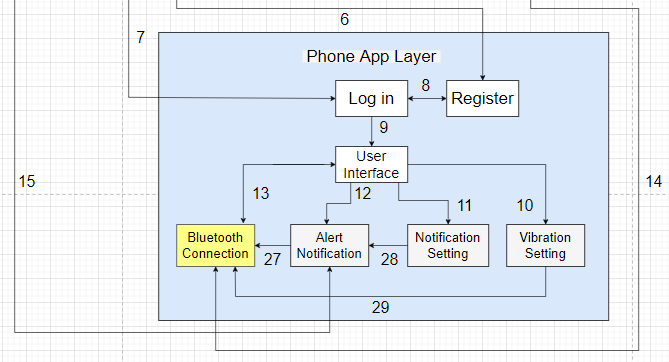
\includegraphics[width=0.60\textwidth]{images/phone_bluetooth.png}
 \caption{Phone App Layer diagram}
\end{figure}

\subsubsection{Assumptions}
It is assumed that the user is already signed in.

\subsubsection{Responsibilities}
This subsystem is responsible for letting users to set up Bluetooth and connect with their wristband module.

\subsubsection{Subsystem Interfaces}
Each of the inputs and outputs for the subsystem are defined here. Create a table with an entry for each labelled interface that connects to this subsystem. For each entry, describe any incoming and outgoing data elements will pass through this interface.

\begin {table}[H]
\caption {Bluetooth Settings interfaces} 
\begin{center}
    \begin{tabular}{ | p{1cm} | p{6cm} | p{3cm} | p{3cm} |}
    \hline
    ID & Description & Inputs & Outputs \\ \hline
    #29 & From vibration setting & \pbox{From vibration setting page} & \pbox{To Bluetooth setting}  \\ \hline
    #27 & From alert notification page & \pbox{From alert notification page} & \pbox{To Bluetooth setting}  \\ \hline
    #14 & Bluetooth setting & \pbox{Switch on and off} & \pbox{Bluetooth turns on and off}  \\ \hline
    #13 & To previous page & \pbox{Click on the back arrow} & \pbox{Main page}  \\ \hline
    \end{tabular}
\end{center}
\end{table}

\subsection{Alert notification}
The alert notification subsystem will allow users to view history on every past alert.

\begin{figure}[h!]
	\centering
 	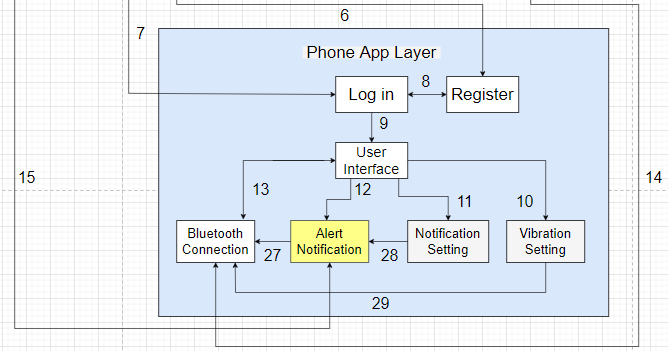
\includegraphics[width=0.60\textwidth]{images/phone_alert.png}
 \caption{Phone App Layer diagram}
\end{figure}

\subsubsection{Assumptions}
It is assumed that the user is already signed in.

\subsubsection{Responsibilities}
This subsystem will record and show all the past alerts on windows and doors. 

\subsubsection{Subsystem Interfaces}
Each of the inputs and outputs for the subsystem are defined here. Create a table with an entry for each labelled interface that connects to this subsystem. For each entry, describe any incoming and outgoing data elements will pass through this interface.

\begin {table}[H]
\caption {Alert notifications interfaces} 
\begin{center}
    \begin{tabular}{ | p{1cm} | p{6cm} | p{3cm} | p{3cm} |}
    \hline
    ID & Description & Inputs & Outputs \\ \hline
    #28 & From notification setting & \pbox{From notification setting} & \pbox{To alert notification}  \\ \hline
    #12 & To previous page & \pbox{Click on the back arrow} & \pbox{Main page}  \\ \hline
    #27 & To Bluetooth connection & \pbox{Click on the 'Bluetooth setting'} & \pbox{Bluetooth setting}  \\ \hline
    \end{tabular}
\end{center}
\end{table}

\subsection{Notification setting}
The notification setting interface subsystem will allow users to change settings for alarm notification.

\begin{figure}[h!]
	\centering
 	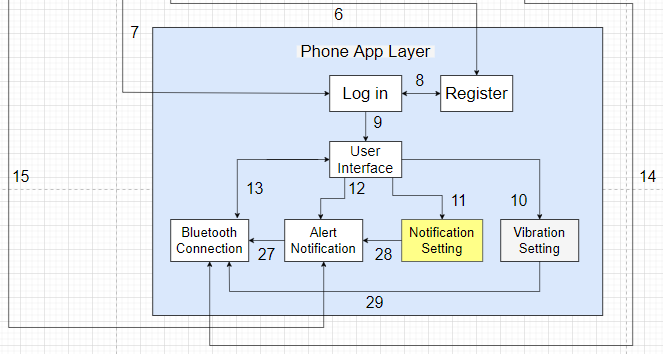
\includegraphics[width=0.60\textwidth]{images/phone_notification.png}
 \caption{Phone App Layer diagram}
\end{figure}

\subsubsection{Assumptions}
It is assumed that the user is already signed in.

\subsubsection{Responsibilities}
This subsystem will allow users to add or remove alerts for each window and the door.

\subsubsection{Subsystem Interfaces}
Each of the inputs and outputs for the subsystem are defined here. Create a table with an entry for each labelled interface that connects to this subsystem. For each entry, describe any incoming and outgoing data elements will pass through this interface.

\begin {table}[H]
\caption {Notification setting interfaces} 
\begin{center}
    \begin{tabular}{ | p{1cm} | p{6cm} | p{3cm} | p{3cm} |}
    \hline
    ID & Description & Inputs & Outputs \\ \hline
    #28 & Move to alert notification & \pbox{Click on the 'Alert notification'} & \pbox{Alert notification page}  \\ \hline
    #11 & To previous page & \pbox{Click on the back arrow} & \pbox{Main page}  \\ \hline
    \end{tabular}
\end{center}
\end{table}

\subsection{Vibration setting}
The notification setting interface subsystem will allow users to change vibration pattern as a notification.

\begin{figure}[h!]
	\centering
 	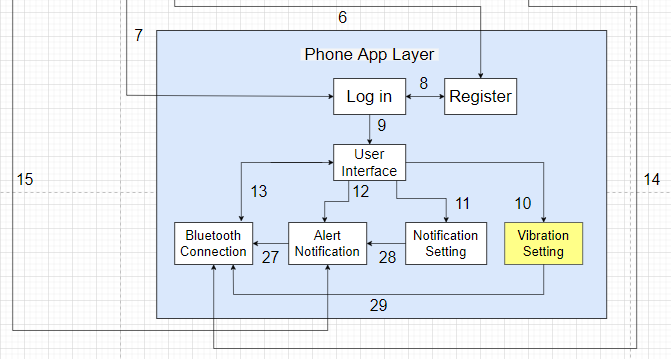
\includegraphics[width=0.60\textwidth]{images/phone_vibration.png}
 \caption{Phone App Layer diagram}
\end{figure}

\subsubsection{Assumptions}
It is assumed that the user is already signed in.

\subsubsection{Responsibilities}
This subsystem will allow users to change vibration patterns in a favor of users. For instance, the essential alert will vibrate stronger.

\subsubsection{Subsystem Interfaces}
Each of the inputs and outputs for the subsystem are defined here. Create a table with an entry for each labelled interface that connects to this subsystem. For each entry, describe any incoming and outgoing data elements will pass through this interface.

\begin {table}[H]
\caption {Vibration setting interfaces} 
\begin{center}
    \begin{tabular}{ | p{1cm} | p{6cm} | p{3cm} | p{3cm} |}
    \hline
    ID & Description & Inputs & Outputs \\ \hline
    #29 & Move to Bluetooth connection setting & \pbox{Click on 'Bluetooth'} & \pbox{Bluetooth page}  \\ \hline
    #10 & To previous page & \pbox{Click on the back arrow} & \pbox{Main page}  \\ \hline
    \end{tabular}
\end{center}
\end{table}